% Options for packages loaded elsewhere
\PassOptionsToPackage{unicode}{hyperref}
\PassOptionsToPackage{hyphens}{url}
%
\documentclass[
  english,
  man, fleqn, noextraspace]{apa6}
\usepackage{lmodern}
\usepackage{amssymb,amsmath}
\usepackage{ifxetex,ifluatex}
\ifnum 0\ifxetex 1\fi\ifluatex 1\fi=0 % if pdftex
  \usepackage[T1]{fontenc}
  \usepackage[utf8]{inputenc}
  \usepackage{textcomp} % provide euro and other symbols
\else % if luatex or xetex
  \usepackage{unicode-math}
  \defaultfontfeatures{Scale=MatchLowercase}
  \defaultfontfeatures[\rmfamily]{Ligatures=TeX,Scale=1}
\fi
% Use upquote if available, for straight quotes in verbatim environments
\IfFileExists{upquote.sty}{\usepackage{upquote}}{}
\IfFileExists{microtype.sty}{% use microtype if available
  \usepackage[]{microtype}
  \UseMicrotypeSet[protrusion]{basicmath} % disable protrusion for tt fonts
}{}
\makeatletter
\@ifundefined{KOMAClassName}{% if non-KOMA class
  \IfFileExists{parskip.sty}{%
    \usepackage{parskip}
  }{% else
    \setlength{\parindent}{0pt}
    \setlength{\parskip}{6pt plus 2pt minus 1pt}}
}{% if KOMA class
  \KOMAoptions{parskip=half}}
\makeatother
\usepackage{xcolor}
\IfFileExists{xurl.sty}{\usepackage{xurl}}{} % add URL line breaks if available
\IfFileExists{bookmark.sty}{\usepackage{bookmark}}{\usepackage{hyperref}}
\hypersetup{
  pdftitle={EDLD 651 Final Project Draft},
  pdfauthor={Anwesha Guha1, Heidi Iwashita1, Christopher Loan1, Adam Nielsen1, \& Aaron Rothbart1},
  pdflang={en-EN},
  pdfkeywords={keywords},
  hidelinks,
  pdfcreator={LaTeX via pandoc}}
\urlstyle{same} % disable monospaced font for URLs
\usepackage{color}
\usepackage{fancyvrb}
\newcommand{\VerbBar}{|}
\newcommand{\VERB}{\Verb[commandchars=\\\{\}]}
\DefineVerbatimEnvironment{Highlighting}{Verbatim}{commandchars=\\\{\}}
% Add ',fontsize=\small' for more characters per line
\usepackage{framed}
\definecolor{shadecolor}{RGB}{248,248,248}
\newenvironment{Shaded}{\begin{snugshade}}{\end{snugshade}}
\newcommand{\AlertTok}[1]{\textcolor[rgb]{0.94,0.16,0.16}{#1}}
\newcommand{\AnnotationTok}[1]{\textcolor[rgb]{0.56,0.35,0.01}{\textbf{\textit{#1}}}}
\newcommand{\AttributeTok}[1]{\textcolor[rgb]{0.77,0.63,0.00}{#1}}
\newcommand{\BaseNTok}[1]{\textcolor[rgb]{0.00,0.00,0.81}{#1}}
\newcommand{\BuiltInTok}[1]{#1}
\newcommand{\CharTok}[1]{\textcolor[rgb]{0.31,0.60,0.02}{#1}}
\newcommand{\CommentTok}[1]{\textcolor[rgb]{0.56,0.35,0.01}{\textit{#1}}}
\newcommand{\CommentVarTok}[1]{\textcolor[rgb]{0.56,0.35,0.01}{\textbf{\textit{#1}}}}
\newcommand{\ConstantTok}[1]{\textcolor[rgb]{0.00,0.00,0.00}{#1}}
\newcommand{\ControlFlowTok}[1]{\textcolor[rgb]{0.13,0.29,0.53}{\textbf{#1}}}
\newcommand{\DataTypeTok}[1]{\textcolor[rgb]{0.13,0.29,0.53}{#1}}
\newcommand{\DecValTok}[1]{\textcolor[rgb]{0.00,0.00,0.81}{#1}}
\newcommand{\DocumentationTok}[1]{\textcolor[rgb]{0.56,0.35,0.01}{\textbf{\textit{#1}}}}
\newcommand{\ErrorTok}[1]{\textcolor[rgb]{0.64,0.00,0.00}{\textbf{#1}}}
\newcommand{\ExtensionTok}[1]{#1}
\newcommand{\FloatTok}[1]{\textcolor[rgb]{0.00,0.00,0.81}{#1}}
\newcommand{\FunctionTok}[1]{\textcolor[rgb]{0.00,0.00,0.00}{#1}}
\newcommand{\ImportTok}[1]{#1}
\newcommand{\InformationTok}[1]{\textcolor[rgb]{0.56,0.35,0.01}{\textbf{\textit{#1}}}}
\newcommand{\KeywordTok}[1]{\textcolor[rgb]{0.13,0.29,0.53}{\textbf{#1}}}
\newcommand{\NormalTok}[1]{#1}
\newcommand{\OperatorTok}[1]{\textcolor[rgb]{0.81,0.36,0.00}{\textbf{#1}}}
\newcommand{\OtherTok}[1]{\textcolor[rgb]{0.56,0.35,0.01}{#1}}
\newcommand{\PreprocessorTok}[1]{\textcolor[rgb]{0.56,0.35,0.01}{\textit{#1}}}
\newcommand{\RegionMarkerTok}[1]{#1}
\newcommand{\SpecialCharTok}[1]{\textcolor[rgb]{0.00,0.00,0.00}{#1}}
\newcommand{\SpecialStringTok}[1]{\textcolor[rgb]{0.31,0.60,0.02}{#1}}
\newcommand{\StringTok}[1]{\textcolor[rgb]{0.31,0.60,0.02}{#1}}
\newcommand{\VariableTok}[1]{\textcolor[rgb]{0.00,0.00,0.00}{#1}}
\newcommand{\VerbatimStringTok}[1]{\textcolor[rgb]{0.31,0.60,0.02}{#1}}
\newcommand{\WarningTok}[1]{\textcolor[rgb]{0.56,0.35,0.01}{\textbf{\textit{#1}}}}
\usepackage{graphicx,grffile}
\makeatletter
\def\maxwidth{\ifdim\Gin@nat@width>\linewidth\linewidth\else\Gin@nat@width\fi}
\def\maxheight{\ifdim\Gin@nat@height>\textheight\textheight\else\Gin@nat@height\fi}
\makeatother
% Scale images if necessary, so that they will not overflow the page
% margins by default, and it is still possible to overwrite the defaults
% using explicit options in \includegraphics[width, height, ...]{}
\setkeys{Gin}{width=\maxwidth,height=\maxheight,keepaspectratio}
% Set default figure placement to htbp
\makeatletter
\def\fps@figure{htbp}
\makeatother
\setlength{\emergencystretch}{3em} % prevent overfull lines
\providecommand{\tightlist}{%
  \setlength{\itemsep}{0pt}\setlength{\parskip}{0pt}}
\setcounter{secnumdepth}{-\maxdimen} % remove section numbering
% Make \paragraph and \subparagraph free-standing
\ifx\paragraph\undefined\else
  \let\oldparagraph\paragraph
  \renewcommand{\paragraph}[1]{\oldparagraph{#1}\mbox{}}
\fi
\ifx\subparagraph\undefined\else
  \let\oldsubparagraph\subparagraph
  \renewcommand{\subparagraph}[1]{\oldsubparagraph{#1}\mbox{}}
\fi
% Manuscript styling
\usepackage{upgreek}
\captionsetup{font=singlespacing,justification=justified}

% Table formatting
\usepackage{longtable}
\usepackage{lscape}
% \usepackage[counterclockwise]{rotating}   % Landscape page setup for large tables
\usepackage{multirow}		% Table styling
\usepackage{tabularx}		% Control Column width
\usepackage[flushleft]{threeparttable}	% Allows for three part tables with a specified notes section
\usepackage{threeparttablex}            % Lets threeparttable work with longtable

% Create new environments so endfloat can handle them
% \newenvironment{ltable}
%   {\begin{landscape}\begin{center}\begin{threeparttable}}
%   {\end{threeparttable}\end{center}\end{landscape}}
\newenvironment{lltable}{\begin{landscape}\begin{center}\begin{ThreePartTable}}{\end{ThreePartTable}\end{center}\end{landscape}}

% Enables adjusting longtable caption width to table width
% Solution found at http://golatex.de/longtable-mit-caption-so-breit-wie-die-tabelle-t15767.html
\makeatletter
\newcommand\LastLTentrywidth{1em}
\newlength\longtablewidth
\setlength{\longtablewidth}{1in}
\newcommand{\getlongtablewidth}{\begingroup \ifcsname LT@\roman{LT@tables}\endcsname \global\longtablewidth=0pt \renewcommand{\LT@entry}[2]{\global\advance\longtablewidth by ##2\relax\gdef\LastLTentrywidth{##2}}\@nameuse{LT@\roman{LT@tables}} \fi \endgroup}

% \setlength{\parindent}{0.5in}
% \setlength{\parskip}{0pt plus 0pt minus 0pt}

% \usepackage{etoolbox}
\makeatletter
\patchcmd{\HyOrg@maketitle}
  {\section{\normalfont\normalsize\abstractname}}
  {\section*{\normalfont\normalsize\abstractname}}
  {}{\typeout{Failed to patch abstract.}}
\patchcmd{\HyOrg@maketitle}
  {\section{\protect\normalfont{\@title}}}
  {\section*{\protect\normalfont{\@title}}}
  {}{\typeout{Failed to patch title.}}
\makeatother
\shorttitle{Final\_Draft}
\keywords{keywords\newline\indent Word count: X}
\DeclareDelayedFloatFlavor{ThreePartTable}{table}
\DeclareDelayedFloatFlavor{lltable}{table}
\DeclareDelayedFloatFlavor*{longtable}{table}
\makeatletter
\renewcommand{\efloat@iwrite}[1]{\immediate\expandafter\protected@write\csname efloat@post#1\endcsname{}}
\makeatother
\usepackage{lineno}

\linenumbers
\usepackage{csquotes}
\raggedbottom
\setlength{\parskip}{0pt}
\ifxetex
  % Load polyglossia as late as possible: uses bidi with RTL langages (e.g. Hebrew, Arabic)
  \usepackage{polyglossia}
  \setmainlanguage[]{english}
\else
  \usepackage[shorthands=off,main=english]{babel}
\fi

\title{EDLD 651 Final Project Draft}
\author{Anwesha Guha\textsuperscript{1}, Heidi Iwashita\textsuperscript{1}, Christopher Loan\textsuperscript{1}, Adam Nielsen\textsuperscript{1}, \& Aaron Rothbart\textsuperscript{1}}
\date{}


\authornote{

All work done herein represents contributions from all authors equally. Author order is alphabetical.

}

\affiliation{\vspace{0.5cm}\textsuperscript{1} University of Oregon}

\abstract{
FILL IN ABSTRACT IF WANTED
}



\begin{document}
\maketitle

\hypertarget{introduction}{%
\section{Introduction}\label{introduction}}

We explore proportion of graduation (outcome), across several categorical variables. In particular, we plan to focus on English learners vs.~English proficient students.

Not only will we report these outcomes across different groups, we will also explore these across boroughs, too, to see if English learners are successing equally across boroughs, compared to the English proficient students in their boroughs.

\hypertarget{methods}{%
\section{Methods}\label{methods}}

Data was taken from INSERT LINK

\hypertarget{participants}{%
\subsection{Participants}\label{participants}}

Explain participants' from what we have in data.

\begin{Shaded}
\begin{Highlighting}[]
\CommentTok{#clean names done here}
\NormalTok{grad <-}\StringTok{ }\KeywordTok{import}\NormalTok{(}\KeywordTok{here}\NormalTok{(}\StringTok{"data"}\NormalTok{, }\StringTok{"2005-2010__Graduation_Outcomes_-__By_Borough.csv"}\NormalTok{))}
\NormalTok{grad <-}\StringTok{ }\NormalTok{grad }\OperatorTok\StringTok{ }
\StringTok{  }\KeywordTok{clean_names}\NormalTok{() }\OperatorTok\StringTok{ }
\StringTok{  }\KeywordTok{as_tibble}\NormalTok{()}

\KeywordTok{summary}\NormalTok{(grad}\OperatorTok{$}\NormalTok{cohort) }\CommentTok{# needs to be cleaned in new df, change Aug 2006 to 2006}
\end{Highlighting}
\end{Shaded}

\begin{verbatim}
##    Length     Class      Mode 
##       385 character character
\end{verbatim}

\begin{Shaded}
\begin{Highlighting}[]
\NormalTok{clean_grad <-}\StringTok{ }\NormalTok{grad}
\NormalTok{clean_grad}\OperatorTok{$}\NormalTok{cohort <-}\StringTok{  }\KeywordTok{as.numeric}\NormalTok{(}\KeywordTok{sub}\NormalTok{(}\StringTok{"Aug 2006"}\NormalTok{, }\StringTok{"2006"}\NormalTok{, grad}\OperatorTok{$}\NormalTok{cohort))}

\NormalTok{clean_grad}
\end{Highlighting}
\end{Shaded}

\begin{verbatim}
## # A tibble: 385 x 22
##    demographic borough cohort total_cohort total_grads_n total_grads_per~
##    <chr>       <chr>    <dbl>        <int>         <int>            <dbl>
##  1 Borough To~ Bronx     2001        11453          4913             42.9
##  2 Borough To~ Bronx     2002        12032          5328             44.3
##  3 Borough To~ Bronx     2003        13632          6389             46.9
##  4 Borough To~ Bronx     2004        14364          7448             51.9
##  5 Borough To~ Bronx     2005        15175          8229             54.2
##  6 Borough To~ Bronx     2006        15579          8524             54.7
##  7 Borough To~ Bronx     2006        15579          9215             59.2
##  8 Borough To~ Brookl~   2001        19961          9758             48.9
##  9 Borough To~ Brookl~   2002        20808         10337             49.7
## 10 Borough To~ Brookl~   2003        21334         11064             51.9
## # ... with 375 more rows, and 16 more variables: total_regents_n <int>,
## #   total_regents_percent_of_cohort <dbl>,
## #   total_regents_percent_of_grads <dbl>, advanced_regents_n <int>,
## #   advanced_regents_percent_of_cohort <dbl>,
## #   advanced_regents_percent_of_grads <dbl>, regents_w_o_advanced_n <int>,
## #   regents_w_o_advanced_percent_of_cohort <dbl>,
## #   regents_w_o_advanced_percent_of_grads <dbl>, local_n <int>,
## #   local_percent_of_cohort <dbl>, local_percent_of_grads <dbl>,
## #   still_enrolled_n <int>, still_enrolled_percent_of_cohort <dbl>,
## #   dropped_out_n <int>, dropped_out_percent_of_cohort <dbl>
\end{verbatim}

\hypertarget{pivots}{%
\subsection{PIVOTS}\label{pivots}}

The data we are starting with are already tidy, but for the purposes of demonstrating our rather acute proficiency in our \emph{ability} to tidy data, in this segment will make the data untidy and then tidy it once more.

\begin{Shaded}
\begin{Highlighting}[]
\NormalTok{messy_grad <-}\StringTok{ }\NormalTok{clean_grad }\OperatorTok\StringTok{ }
\StringTok{  }\KeywordTok{pivot_wider}\NormalTok{(}\DataTypeTok{names_from =}\NormalTok{ borough,}
              \DataTypeTok{values_from =}\NormalTok{ total_cohort)}
\NormalTok{messy_grad}
\end{Highlighting}
\end{Shaded}

\begin{verbatim}
## # A tibble: 385 x 25
##    demographic cohort total_grads_n total_grads_per~ total_regents_n
##    <chr>        <dbl>         <int>            <dbl>           <int>
##  1 Borough To~   2001          4913             42.9            2644
##  2 Borough To~   2002          5328             44.3            3118
##  3 Borough To~   2003          6389             46.9            3861
##  4 Borough To~   2004          7448             51.9            4625
##  5 Borough To~   2005          8229             54.2            5618
##  6 Borough To~   2006          8524             54.7            6312
##  7 Borough To~   2006          9215             59.2            6605
##  8 Borough To~   2001          9758             48.9            6177
##  9 Borough To~   2002         10337             49.7            7050
## 10 Borough To~   2003         11064             51.9            7711
## # ... with 375 more rows, and 20 more variables:
## #   total_regents_percent_of_cohort <dbl>,
## #   total_regents_percent_of_grads <dbl>, advanced_regents_n <int>,
## #   advanced_regents_percent_of_cohort <dbl>,
## #   advanced_regents_percent_of_grads <dbl>, regents_w_o_advanced_n <int>,
## #   regents_w_o_advanced_percent_of_cohort <dbl>,
## #   regents_w_o_advanced_percent_of_grads <dbl>, local_n <int>,
## #   local_percent_of_cohort <dbl>, local_percent_of_grads <dbl>,
## #   still_enrolled_n <int>, still_enrolled_percent_of_cohort <dbl>,
## #   dropped_out_n <int>, dropped_out_percent_of_cohort <dbl>, Bronx <int>,
## #   Brooklyn <int>, Manhattan <int>, Queens <int>, `Staten Island` <int>
\end{verbatim}

\begin{Shaded}
\begin{Highlighting}[]
\NormalTok{clean_grad_}\DecValTok{2}\NormalTok{ <-}\StringTok{ }\NormalTok{messy_grad }\OperatorTok\StringTok{ }
\StringTok{  }\KeywordTok{pivot_longer}\NormalTok{(}\DataTypeTok{cols =} \KeywordTok{c}\NormalTok{(}\StringTok{"Bronx"}\OperatorTok{:}\StringTok{"Staten Island"}\NormalTok{),}
               \DataTypeTok{names_to =} \StringTok{"borough"}\NormalTok{,}
               \DataTypeTok{values_to =} \StringTok{"total_cohort"}\NormalTok{,}
               \DataTypeTok{values_drop_na =} \OtherTok{TRUE}\NormalTok{)}

\NormalTok{clean_grad_}\DecValTok{2}\NormalTok{ <-}\StringTok{ }\NormalTok{clean_grad_}\DecValTok{2}\NormalTok{[, }\KeywordTok{c}\NormalTok{(}\DecValTok{1}\NormalTok{,}\DecValTok{21}\NormalTok{,}\DecValTok{2}\NormalTok{,}\DecValTok{22}\NormalTok{,}\DecValTok{3}\OperatorTok{:}\DecValTok{20}\NormalTok{)]}
\NormalTok{clean_grad_}\DecValTok{2}
\end{Highlighting}
\end{Shaded}

\begin{verbatim}
## # A tibble: 385 x 22
##    demographic borough cohort total_cohort total_grads_n total_grads_per~
##    <chr>       <chr>    <dbl>        <int>         <int>            <dbl>
##  1 Borough To~ Bronx     2001        11453          4913             42.9
##  2 Borough To~ Bronx     2002        12032          5328             44.3
##  3 Borough To~ Bronx     2003        13632          6389             46.9
##  4 Borough To~ Bronx     2004        14364          7448             51.9
##  5 Borough To~ Bronx     2005        15175          8229             54.2
##  6 Borough To~ Bronx     2006        15579          8524             54.7
##  7 Borough To~ Bronx     2006        15579          9215             59.2
##  8 Borough To~ Brookl~   2001        19961          9758             48.9
##  9 Borough To~ Brookl~   2002        20808         10337             49.7
## 10 Borough To~ Brookl~   2003        21334         11064             51.9
## # ... with 375 more rows, and 16 more variables: total_regents_n <int>,
## #   total_regents_percent_of_cohort <dbl>,
## #   total_regents_percent_of_grads <dbl>, advanced_regents_n <int>,
## #   advanced_regents_percent_of_cohort <dbl>,
## #   advanced_regents_percent_of_grads <dbl>, regents_w_o_advanced_n <int>,
## #   regents_w_o_advanced_percent_of_cohort <dbl>,
## #   regents_w_o_advanced_percent_of_grads <dbl>, local_n <int>,
## #   local_percent_of_cohort <dbl>, local_percent_of_grads <dbl>,
## #   still_enrolled_n <int>, still_enrolled_percent_of_cohort <dbl>,
## #   dropped_out_n <int>, dropped_out_percent_of_cohort <dbl>
\end{verbatim}

\begin{Shaded}
\begin{Highlighting}[]
\CommentTok{#select() relevant variables to make subsetted dataset}
\CommentTok{#filter() out cases that are of interest }
\end{Highlighting}
\end{Shaded}

\begin{Shaded}
\begin{Highlighting}[]
\CommentTok{#descriptive stats (counts of demographics reported by borough in a table() call?) we don't have much info here}
\end{Highlighting}
\end{Shaded}

\hypertarget{data-analysis}{%
\subsection{Data analysis}\label{data-analysis}}

All analysis were conducted in R, with heavy reliance upon the \texttt{\{tidyverse\}} packages to manipulate and visualize the data.

\hypertarget{results}{%
\section{Results}\label{results}}

\begin{Shaded}
\begin{Highlighting}[]
\CommentTok{#group_by() }
\CommentTok{#summarize() }
\CommentTok{#report graduation by borough}
\CommentTok{#report graduation by english language status}
\CommentTok{#report graduation by borough & english learner status}
\end{Highlighting}
\end{Shaded}

\begin{Shaded}
\begin{Highlighting}[]
\CommentTok{#Chris Loan would like to do this part: graphing. }
\CommentTok{# my code works assuming we use the "clean_grad" dataset in the `final_project.Rmd` file. You can get it to run there.}

\CommentTok{#graph outcomes by English language status}
\CommentTok{#facet wrap by borough}
\CommentTok{#jitter the points so we can see all the years}
\CommentTok{#give color to all the years so we can differentiate them}

\NormalTok{clean_grad }\OperatorTok\StringTok{ }
\StringTok{  }\KeywordTok{filter}\NormalTok{(demographic }\OperatorTok{==}\StringTok{ "English Language Learners"} \OperatorTok{|}\StringTok{ }
\StringTok{           }\NormalTok{demographic }\OperatorTok{==}\StringTok{ "English Proficient Students"}\NormalTok{) }\OperatorTok\StringTok{ }
\StringTok{  }\KeywordTok{mutate}\NormalTok{(}\StringTok{`}\DataTypeTok{English Language Learner Status}\StringTok{`}\NormalTok{ =}\StringTok{ }
\StringTok{           }\KeywordTok{factor}\NormalTok{(demographic, }
                  \DataTypeTok{levels =} \KeywordTok{c}\NormalTok{(}\StringTok{"English Language Learners"}\NormalTok{, }
                      \StringTok{"English Proficient Students"}\NormalTok{), }
                  \DataTypeTok{labels =} \KeywordTok{c}\NormalTok{(}\StringTok{'Learner'}\NormalTok{, }\StringTok{'Proficient'}\NormalTok{)}
\NormalTok{                  )}
\NormalTok{         ) }\OperatorTok\StringTok{ }\KeywordTok{group_by}\NormalTok{(}\StringTok{`}\DataTypeTok{English Language Learner Status}\StringTok{`}\NormalTok{, borough) }\OperatorTok\StringTok{ }
\StringTok{  }\KeywordTok{ggplot}\NormalTok{(}\KeywordTok{aes}\NormalTok{(}\DataTypeTok{x =} \StringTok{`}\DataTypeTok{English Language Learner Status}\StringTok{`}\NormalTok{, }
             \DataTypeTok{y =}\NormalTok{ total_grads_percent_of_cohort)) }\OperatorTok{+}
\StringTok{  }\KeywordTok{geom_jitter}\NormalTok{(}\KeywordTok{aes}\NormalTok{(}\DataTypeTok{color =}\NormalTok{ cohort)) }\OperatorTok{+}\StringTok{ }\KeywordTok{facet_wrap}\NormalTok{(}\OperatorTok{~}\NormalTok{borough) }\OperatorTok{+}\StringTok{ }
\StringTok{  }\KeywordTok{labs}\NormalTok{(}\DataTypeTok{title =} \StringTok{'Figure 1. Graduation Rates in NYC by English Learner Status'}\NormalTok{,}
       \DataTypeTok{subtitle =} \StringTok{'Boroughs are reported separetely with lighter dots indicating more recent years'}\NormalTok{,}
       \DataTypeTok{y =} \StringTok{'Percent of total cohort'}\NormalTok{)}
\end{Highlighting}
\end{Shaded}

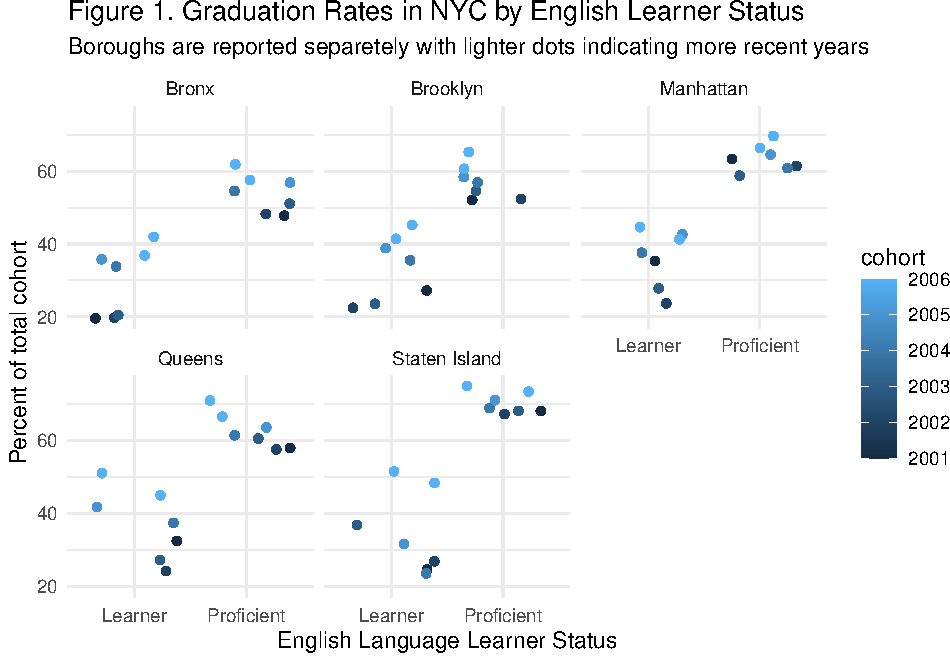
\includegraphics{EDLD_651_Final_Project_Draft_files/figure-latex/graph_results-1.pdf}

\hypertarget{discussion}{%
\section{Discussion}\label{discussion}}

Differences appear to be blah by blah for blah. XYZ boroughs should consider blah blah blah, based on the results. Inferential tests are recommended for next directions.

\newpage

\hypertarget{references}{%
\section{References}\label{references}}

\begingroup
\setlength{\parindent}{-0.5in}
\setlength{\leftskip}{0.5in}

\hypertarget{refs}{}

\endgroup


\end{document}
